\documentclass[12pt, letterpaper]{article}

\usepackage[utf8]{inputenc}
\usepackage{graphicx}
\usepackage{amsmath}
\usepackage[parfill]{parskip}
\usepackage{float}
\usepackage{subfigure}
\usepackage{geometry}
 \geometry{
 a4paper,
 total={160mm,247mm},
 left=25mm,
 top=25mm,
 }
 
\usepackage{hyperref}
\hypersetup{
    colorlinks=true,
    linkcolor=black,
    filecolor=black,      
    urlcolor=blue,
    pdftitle={Linear Interpolator Documentation},
    pdfpagemode=FullScreen,
}
    
\urlstyle{same}

\title{\textbf{Linear Interpolator Documentation}}
\author{Matteo Abaterusso}
\date{\today}

\begin{document}

\begin{titlepage}
	\begin{center}
		\begin{figure}
			
\includegraphics[width=\textwidth]{img/Logo.png}         
		\end{figure}
		{\Large
			Computer Engineering\\
			\vspace{5mm} %5mm vertical space
			Electronic Systems}\\
		\vspace{30mm} %5mm vertical space
		{\Huge\textbf{Linear Interpolator Documentation}}\\
		\vspace{10mm} %5mm vertical space
		{\Large Project Report}\\
		\par\noindent\rule{\textwidth}{0.4pt}
		\begin{flushright}
			%\textbf{TEAM MEMBERS}:\\
			% Cristiano 1\\ 
			% Cristiano 2\\ 
			Matteo Abaterusso\\
			
		\end{flushright}
		\vfill
		Academic Year: 2021/2022\\        
	\end{center}
\end{titlepage} 

\newpage
\tableofcontents

\section{Introduction}

A \textbf{linear interpolator} is a digital circuit that implements the following function:

\begin{displaymath}
    y(nT+uT) = (y_{n+1} - y_n)u + y_n \qquad u=\frac{k}{L}, k \in \{0,1,...,L-1\}
\end{displaymath}

In general, given \textbf{two consecutive input signals} sampled every $T$, the interpolator generates $L$ \textbf{output signals}, with a period of $\frac{T}{L}$ (for this reason $L$ is defined \textbf{factor of interpolation}). If the two input signals represent two points on a cartesian plane, the output signals lie on the line that connects the two inputs.

\subsection{Design Specifications}

The interpolator shall have the following characteristics:

\begin{itemize}
    \item \textbf{Input} and \textbf{output} are represented by 16 bit, so they can assume any integer values between 0 and 65535.
    \item The input signals have a \textbf{sampling period} of $T$, so the circuit will receive every $T$ a new signal.
    \item The factor of interpolation is fixed to $L=4$. So the \textbf{period} with which \textbf{output signals} have to be produced is $\frac{T}{4}$.
\end{itemize}

Moreover the structure of the circuit's \textbf{I/O ports} have to be the following:

\begin{figure}[H]
    \centering
    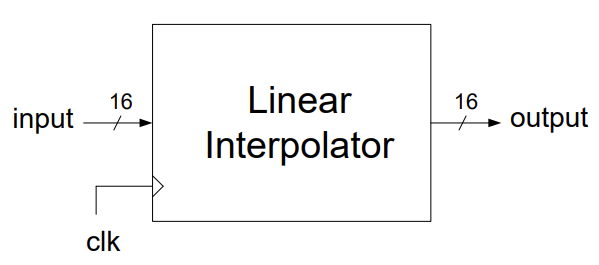
\includegraphics[width=0.5\textwidth]{img/IOPorts.png}
    \caption{Circuit's I/O Ports}
    \label{fig:IOPorts}
\end{figure}

\subsection{Useful Symbols}

The following \textbf{symbol} will be used to identify the signals:

\begin{itemize}
    \item $y_{n+1}$, is the last received signal.
    \item $y_n$, is the second last received signal.
    \item $OUT_i$, is one of the four output signals.
\end{itemize}
\section{Architecture Description}

The first problem to solve is the \textbf{complexity} of the \textbf{operations}. In fact, the linear interpolation requires \textbf{multiplications} and \textbf{divisions}, whose circuits aren't trivial. But in this case the factor interpolation is fixed to $4$, and is a \textbf{power of two}. So is possible for example to exploit the \textbf{shift operation} in base two, to do the division by powers of two in a zero complexity way.

All the \textbf{simplifications} made in the calculation of all outputs are described below:

\[OUT_i = (y_{n+1} - y_n)\frac{i}{4} + y_n = y_{n+1} \frac{i}{4} - y_n \frac{i}{4} + y_n\] 
\[OUT_0 = y_{n+1} \frac{0}{4} - y_n \frac{0}{4} + y_n = y_n\] 
\[OUT_1 = y_{n+1} \frac{1}{4} - y_n \frac{1}{4} + y_n = y_{n+1} \frac{1}{4} + y_n \frac{3}{4} =  y_{n+1} \frac{1}{4} + y_n \frac{2}{4} + y_n \frac{1}{4} = y_{n+1} \frac{1}{4} + y_n \frac{1}{2} + y_n \frac{1}{4}\]
\[OUT_2 = y_{n+1} \frac{2}{4} - y_n \frac{2}{4} + y_n = y_{n+1} \frac{2}{4} + y_n \frac{2}{4} = y_{n+1} \frac{1}{2} + y_n \frac{1}{2}\] 
\[OUT_2 = y_{n+1} \frac{3}{4} - y_n \frac{3}{4} + y_n = y_{n+1} \frac{3}{4} + y_n \frac{1}{4} =  y_{n+1} \frac{1}{4} + y_{n+1} \frac{2}{4} + y_n \frac{1}{4} = y_{n+1} \frac{1}{4} + y_{n+1} \frac{1}{2} + y_n \frac{1}{4}\]

So in conclusion the equations that have to be implemented are:

\[OUT_0 =  y_n\] 
\[OUT_1 = \frac{y_{n+1}}{4} + \frac{y_n}{2} + \frac{y_n}{4}\]
\[OUT_2 = \frac{y_{n+1}}{2} + \frac{y_n}{2}\] 
\[OUT_2 = \frac{y_{n+1}}{4} + \frac{y_{n+1}}{2} + \frac{y_n}{4}\]

It's clear from the equations above that:

\begin{itemize}
    \item There are \textbf{no subtractions}, but only summations, so it is possible to use \textbf{unsigned signals} that can be summed by a Ripple Carry Adder.   
    \item There are \textbf{no multiplications}, but only divisions by powers of two. The signals are unsigned, so they can be implemented by \textbf{bit a bit right shifts}.
\end{itemize}

Using integer signals and divisions that ignores reminder, the results will have some \textbf{error} compared to the original formula. But this is an acceptable error, considering the huge benefits obtained in terms of circuit complexity.

\newpage

\subsection{Block Diagram}

An high level representation of the the circuit is the following:

\begin{figure}[H]
    \centering
    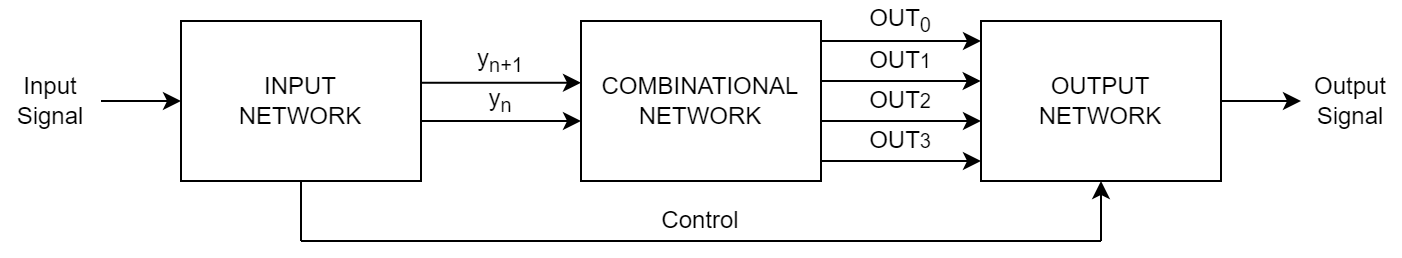
\includegraphics[width=1\textwidth]{img/Chapter2/BlockDiagram.png}
    \caption{Block Diagram}
    \label{fig:BlockDiagram}
\end{figure}

Every block will be analized, starting from the combinational network that performs the calculation of the output signals.

\subsection{Combinational Network}

The combinational network is at the heart of the circuit. Given two signals in input, it provides \textbf{all four interpolated signals}:

\begin{figure}[H]
    \centering
    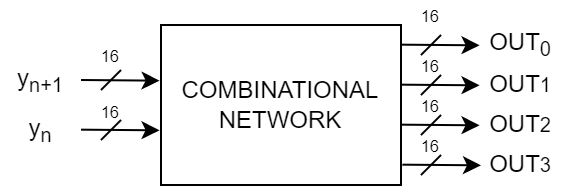
\includegraphics[width=0.6\textwidth]{img/Chapter2/CombinationalIO.png}
    \caption{Combinational Network I/O Ports}
    \label{fig:CNIO}
\end{figure}

The calculations is divided into two parts:

\begin{enumerate}
    \item It compute the \textbf{four signals needed} throw bit a bit shifts ($\frac{y_{n+1}}{4}, \frac{y_{n+1}}{2}, \frac{y_n}{4}, \frac{y_n}{2}$).
    \item It combine the signals obtained with a set of Ripple Carry Adders, to compute the \textbf{final results}.
\end{enumerate}

\newpage

The second point is implemented in this way:

\begin{figure}[H]
    \centering
    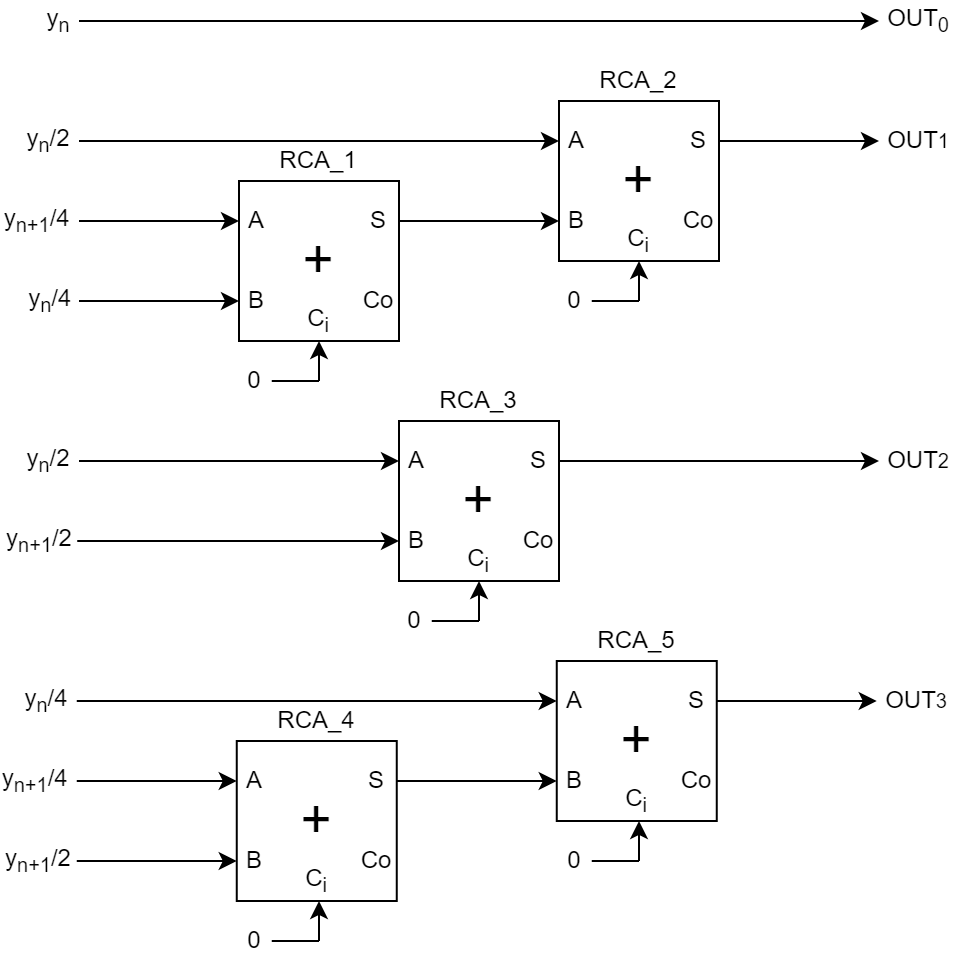
\includegraphics[width=0.6\textwidth]{img/Chapter2/CombinationalStructure.png}
    \caption{Output Signals Calculation}
    \label{fig:OutputSignalsCalc}
\end{figure}

So \textbf{five Ripple Carry Adders} are needed.

\subsubsection{The Synchronization Problem}

Before moving to the study of input and output blocks, it is necessary to consider that the frequency with which the output signals have to be produced is \textbf{four time greater} the input signals arrival frequency.

In order to evaluate the \textbf{timing requirements} of the circuit, registers after input and before output are needed (to have always a \textbf{register-logic-register structure}). So it's clear that the output register has to be updated more frequently than the one in input.

The possible solutions to this problem are two:

\begin{itemize}
    \item Implement \textbf{two different clock domains}, one with a period of $T$ and one of $\frac{T}{4}$.
    \item Implement only the fastest clock (the one with a period of $\frac{T}{4}$), and exploit the \textbf{input register enabler port} to memorize a new signal only once every four clock cycles.  
\end{itemize}

It's clear that the first solution offers the best performance, but at very high cost in terms of complexity. So the second solution has been chosen, that as before in the calculation of the output signals, is the \textbf{best trade-off} between performance and design complexity.

Now will be described how this solution has been implemented in the input network.

\subsection{Input Network}

The main purpose of this network is to \textbf{receive} and \textbf{memorize} every period $T$ the \textbf{new signal}, and to \textbf{maintain it stable} for the combinational network. Moreover even the \textbf{second last input} must also be kept stable, because it is required for the interpolation as well.

To do that \textbf{two registers}, composed by 16 \textbf{D Flip Flop}, have been used. The first register (named \textit{REG\_NI}) take in input the \textbf{receiving signal}. The output of this register provides the signal $y_{n+1}$ to the combinational network. Also it goes in input to a second register (named \textit{REG\_OI}). This second register provides to the combinational network the signal $y_n$. In fact, when the clock arrives \textit{REG\_NI} memorizes the new signal from the outside, and \textit{REG\_OI} memorizes the previous value contained in \textit{REG\_NI}.

The network described above looks like this:

\begin{figure}[H]
    \centering
    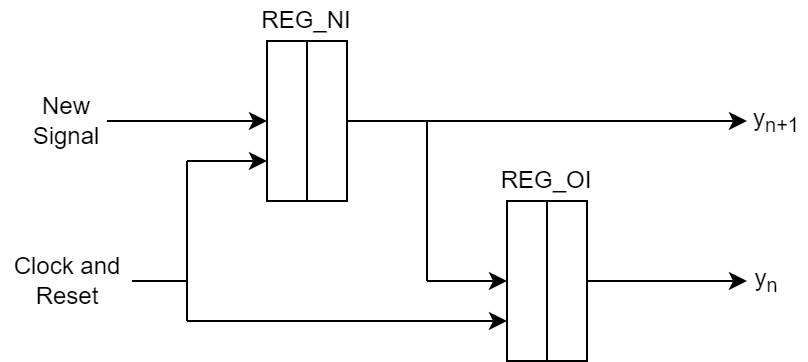
\includegraphics[width=0.5\textwidth]{img/Chapter2/InputNetwork1.png}
    \caption{Input Network Registers}
    \label{fig:InputNetwork1}
\end{figure}

In order to implement the \textbf{synchronization problem solution} (section 2.2.1) is necessary to set the registers enabler port to one every four clock cycle. To do that a \textbf{2 bit counter} has been implemented, the count from 0 to 3, increasing its value of one \textbf{every clock cycle}. Assuming that a new signal arrives when the output of counter is 0, the enabler has to be one in the previous cycle, so when the counter output is 3 ($|11|_2$ in base 2). Therefore, the counter output goes in input to an \textbf{AND port}, whose output becomes the \textbf{enabler line} for the two input registers.

The resulting network is as follows:

\begin{figure}[H]
    \centering
    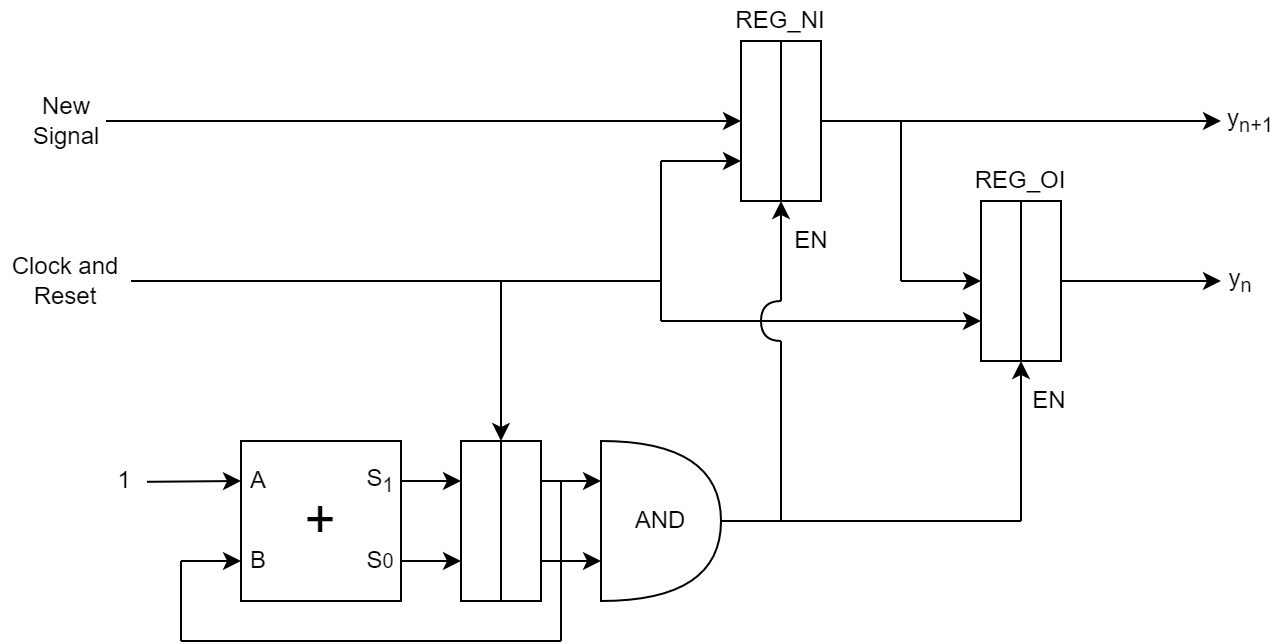
\includegraphics[width=0.65\textwidth]{img/Chapter2/InputNetwork2.png}
    \caption{Total Input Network}
    \label{fig:InputNetwork2}
\end{figure}

So \textbf{one Ripple Carry Adder} and \textbf{three Registers} are needed.

\subsection{Output Network}

The last network of the circuit has to \textbf{output one at a time} the four signals calculated by the combinatorial network. 

To do that a \textbf{multiplexer} has been used. It take in input the four signals resulting from the combinational network and provides them one at time. The output of multiplexer is controlled by the \textbf{counter} of the \textbf{input network}, whose output is exactly a line that change from 0 to 3 every clock cycle.

The output of the multiplexer goes in input to a \textbf{register} (named \textit{REG\_OUT}), whose output is the \textbf{output} of the \textbf{entire circuit}.

The network described above looks like this:

\begin{figure}[H]
    \centering
    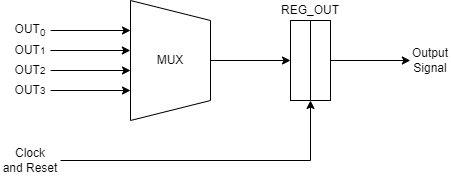
\includegraphics[width=0.7\textwidth]{img/Chapter2/OutputNetwork.png}
    \caption{Output Network}
    \label{fig:OutputNetwork}
\end{figure}

For this last network \textbf{one multiplexer} and \textbf{one register} are needed.
\section{VHDL Code Analysis}

The VHDL analysis will be done through a \textbf{bottom-up approach}. In the first step the basic components will be analyzed, and through them the Linear Interpolator will be obtained.

\subsection{Ripple Carry Adder}

The Ripple Carry Adder is based on the \textbf{Full Adder}, whose implements the sum between two bits, taking into account a possible carry. The Full Adder is defined as follows:

\begin{figure}[H]
    \centering
    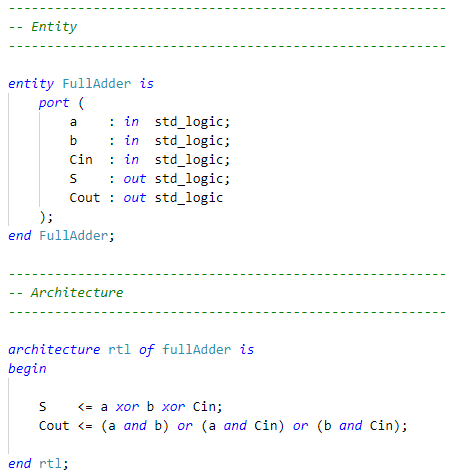
\includegraphics[width=0.5\textwidth]{img/Chapter3/FA.png}
    \caption{Full adder}
    \label{fig:FA}
\end{figure}

So the \textbf{Ripple Carry Adder} consists of a cascade of Full Adder:

\begin{figure}[H]
    \centering
    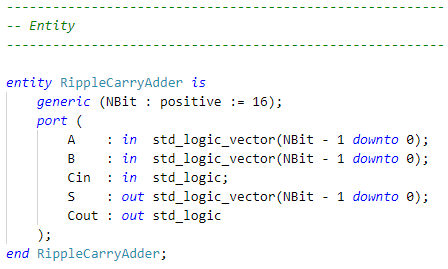
\includegraphics[width=0.5\textwidth]{img/Chapter3/RCA-entity.png}
    \caption{Ripple Carry Adder Entity}
    \label{fig:RCAE}
\end{figure}

\begin{figure}[H]
    \centering
    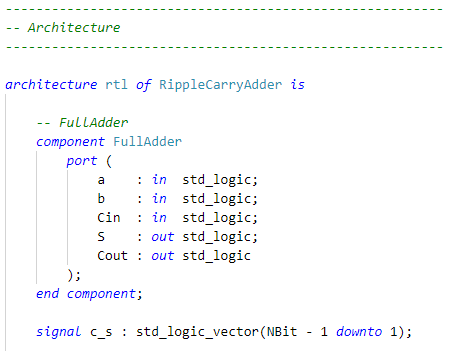
\includegraphics[width=0.5\textwidth]{img/Chapter3/RCA-Architecture1.png}
    \caption{Ripple Carry Adder Component and Signals}
    \label{fig:RCAA1}
\end{figure}

\begin{figure}[H]
    \centering
    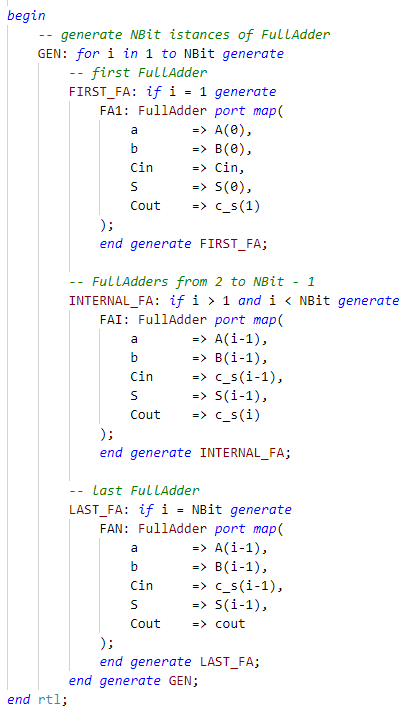
\includegraphics[width=0.5\textwidth]{img/Chapter3/RCA-Architecture2.png}
    \caption{Ripple Carry Adder Internal Architecture}
    \label{fig:RCAA2}
\end{figure}

\subsection{D Flip Flop}

A \textbf{D Flip Flop} involves the use of a low active asynchronous reset. When the clock arrives it stores the new input data only if the enabler is set to one.

\begin{figure}[H]
    \centering
    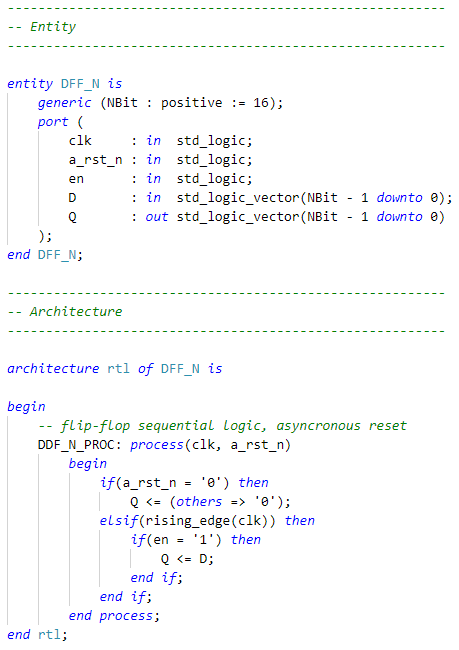
\includegraphics[width=0.5\textwidth]{img/Chapter3/DFF.png}
    \caption{D Flip Flop}
    \label{fig:DFF}
\end{figure}

\subsection{Counter}

The \textbf{Counter} take in input clock and reset, and at every clock cycle it have to increment by one the value that provides in output.

\begin{figure}[H]
    \centering
    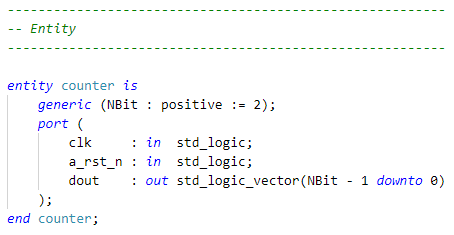
\includegraphics[width=0.5\textwidth]{img/Chapter3/Counter-entity.png}
    \caption{Counter Entity}
    \label{fig:CE}
\end{figure}

Internally it is composed by a register (D Flip Flop) to save and keep stable the output value. The increment operation is implemented through a Ripple Carry Adder. 

\begin{figure}[H]
    \centering
    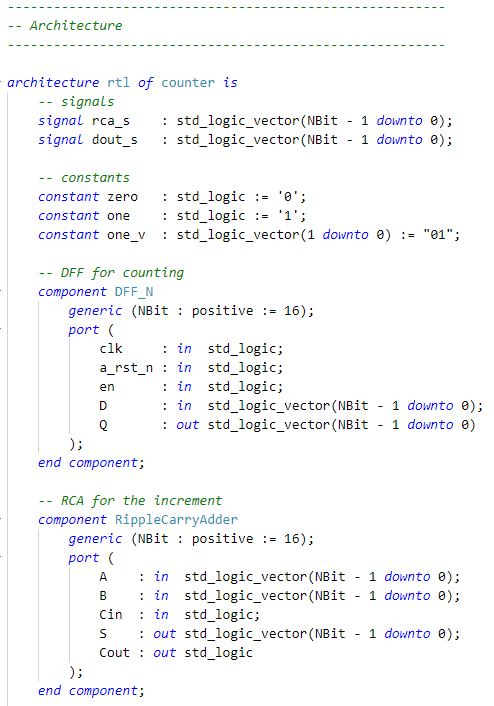
\includegraphics[width=0.5\textwidth]{img/Chapter3/Counter-architecture1.png}
    \caption{Counter Components and Signals}
    \label{fig:CA1}
\end{figure}

The register's output returns in feedback to the Ripple Carry Adder, that sums it to one.

\begin{figure}[H]
    \centering
    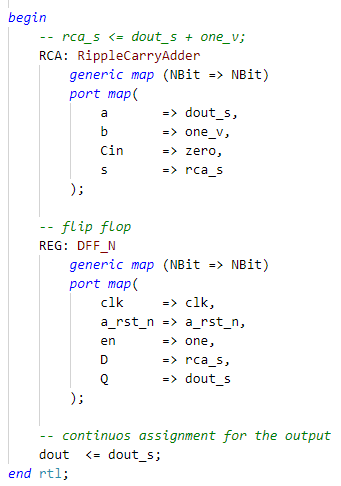
\includegraphics[width=0.4\textwidth]{img/Chapter3/Counter-architecture2.png}
    \caption{Counter Internal Architecture}
    \label{fig:CA2}
\end{figure}

\subsection{Combinational Network}

The \textbf{Combinational Network} follows the structure described in the section 2.2.

\begin{figure}[H]
    \centering
    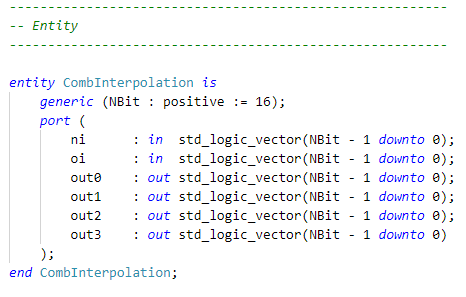
\includegraphics[width=0.5\textwidth]{img/Chapter3/CombInterp-entity.png}
    \caption{Combinational Network Entity}
    \label{fig:CNE}
\end{figure}

As regards the signals, the first four in figure \ref{fig:CNA1} need to implement the divisions by power of two, so they are the signals used by the Ripple Carry Adders to compute the resulting signals.

\begin{figure}[H]
    \centering
    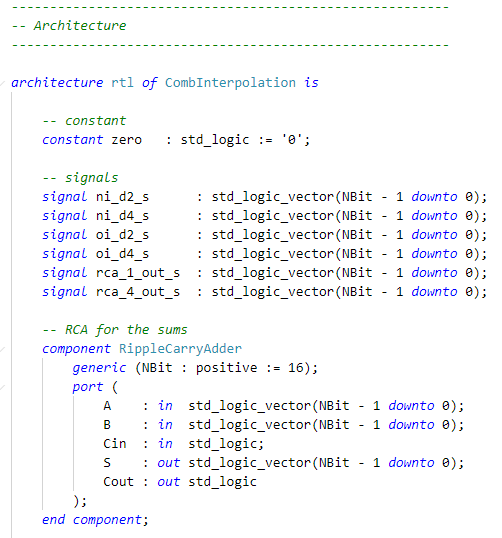
\includegraphics[width=0.5\textwidth]{img/Chapter3/CombInterp-architecture.png}
    \caption{Combinational Network Components and Signals}
    \label{fig:CNA1}
\end{figure}

The next part implements the calculations of the signals described above ($\frac{y_{n+1}}{4}, \frac{y_{n+1}}{2}, \frac{y_n}{4}, \frac{y_n}{2}$). In fact, a single bit shift to right is carried  out to implement the division by two, and of two bit to implement the division by four.

\begin{figure}[H]
    \centering
    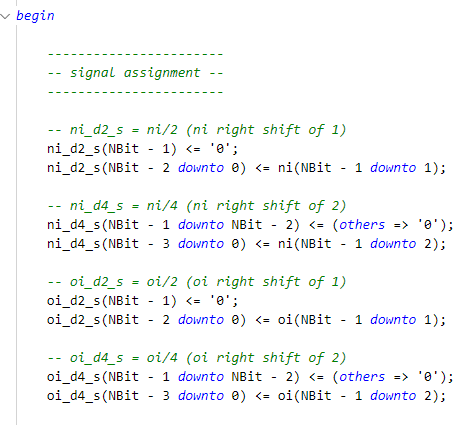
\includegraphics[width=0.5\textwidth]{img/Chapter3/CombInterp-shift.png}
    \caption{Combinational Network Shift bit a bit}
    \label{fig:CNA2}
\end{figure}

The second part of architecture, instead, implements the network described by the figure \ref{fig:OutputSignalsCalc}, that is a composition of five  Ripple Carry Adders, which sums the four signals obtained by the shifts.

\begin{figure}[H]
    \centering
    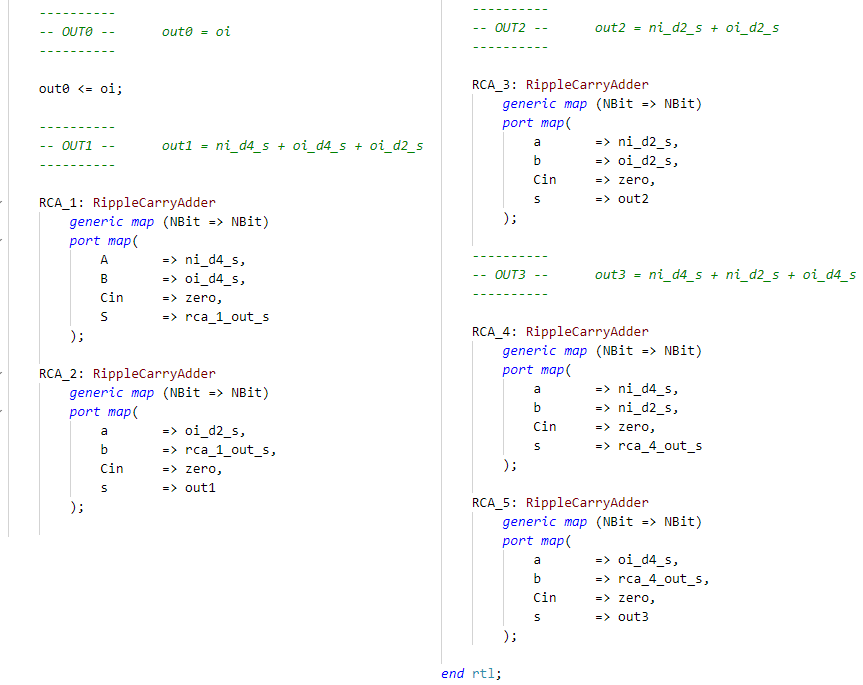
\includegraphics[width=0.8\textwidth]{img/Chapter3/CombInterp-out.png}
    \caption{Combinational Network Output}
    \label{fig:CNA3}
\end{figure}

\newpage

\subsection{Linear Interpolator}

As said before, the \textbf{Linear Interpolator} takes a signals in input and provides in output another signals.

\begin{figure}[H]
    \centering
    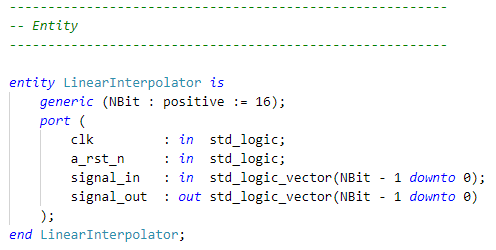
\includegraphics[width=0.5\textwidth]{img/Chapter3/LinearInterpolator-entity.png}
    \caption{Linear Interpolator Entity}
    \label{fig:LIE}
\end{figure}

The Linear Interpolator contains all the previous circuits, so Ripple Carry Adders, D Flip Flops and the Combinational Network.

\begin{figure}[H]
    \centering
    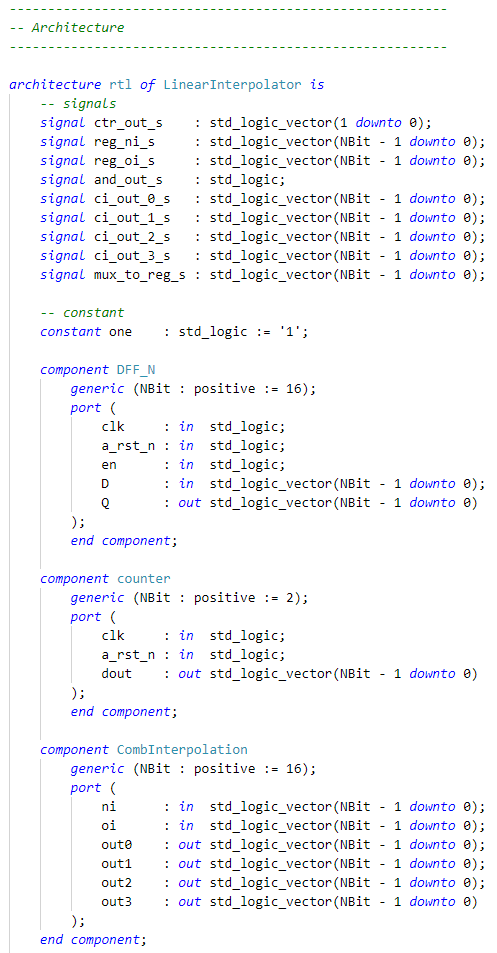
\includegraphics[width=0.45\textwidth]{img/Chapter3/LinearInterpolator-architecture1.png}
    \caption{Linear Interpolator Entity}
    \label{fig:LIA1}
\end{figure}

\textit{REG\_OI} and \textit{REG\_NI} (that are two D Flip Flop), implements the Input Network. In addition to them there is the Counter, whose output go in input to an AND port, implemented by the signal and\_out  \_s. This single bit signal is used as enabler by \textit{REG\_OI} and \textit{REG\_NI}.

The output signals of this two registers are the inputs for the Combinational Network that provides in output the four computed signals. These obtained signals go in input to a Multiplexer, whose output is controlled by the output of the Counter.

The combination between Multiplexer and the register that memorizes its output (\textit{REG\_OUT}) represent the Output Network.

\begin{figure}[H]
    \centering
    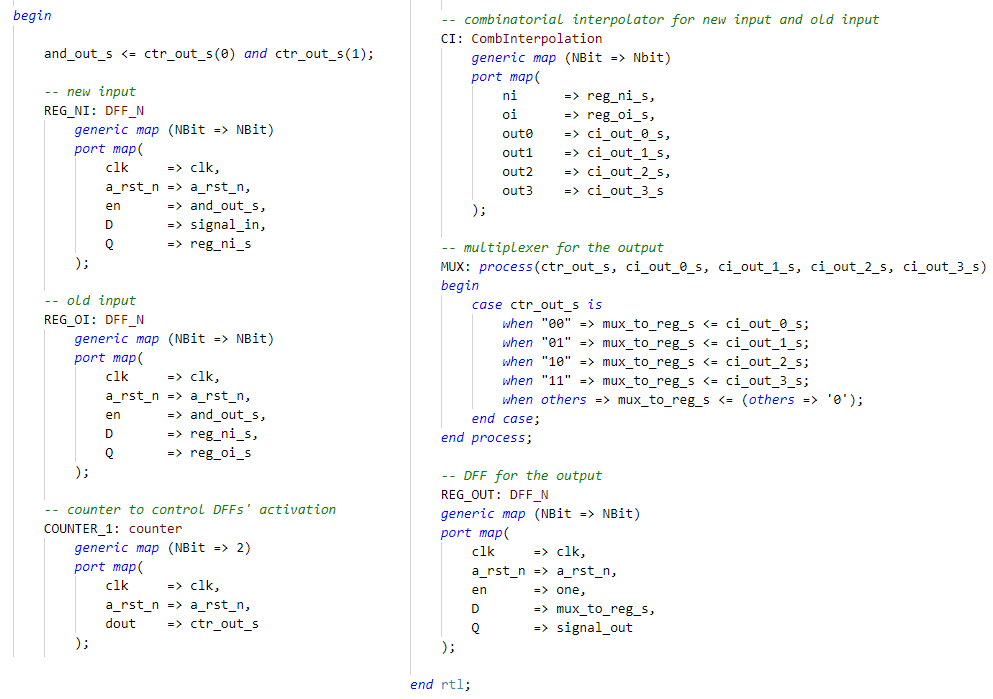
\includegraphics[width=1\textwidth]{img/Chapter3/LinearInterpolator-architecture2.png}
    \caption{Linear Interpolator Entity}
    \label{fig:LIA2}
\end{figure}
\section{Test Plan}

The following steps have been made to test the proper functioning of every part of the Linear Interpolator:

\begin{enumerate}
    \item \textbf{Ripple Carry Adder}, \textbf{D Flip Flop} and \textbf{Counter} have been tested independently, using separate test bench.
    \item The \textbf{Combinational Network} has been tested through comparison with specific values previously decided.
    \item The same values are been used to test the total \textbf{Linear Interpolator}.
    \item Two \textbf{scripts} have been made to test the total circuit with \textbf{signals dynamically generated}.
\end{enumerate}

\subsection{Basic Circuits Test}

The \textbf{Ripple Carry Adder} has been tested by choosing specific values for the input, and checking that the values of outputs represent the right sum and carry out.

\begin{figure}[H]
    \centering
    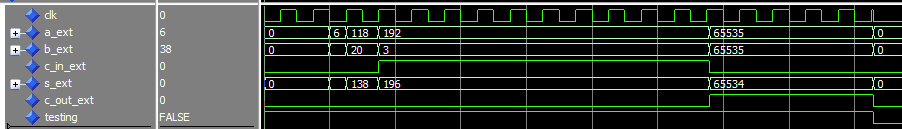
\includegraphics[width=1\textwidth]{img/Chapter4/rca.png}
    \caption{Ripple Carry Adder Test}
    \label{fig:RCATest}
\end{figure}

For the \textbf{D Flip Flop} has been tested the ability to save and keep stable the values received in input. Moreover, has been tested the proper functioning of enabler port.

\begin{figure}[H]
    \centering
    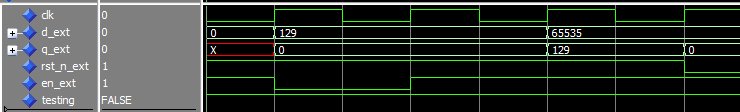
\includegraphics[width=1\textwidth]{img/Chapter4/dff.png}
    \caption{D Flip Flop Test}
    \label{fig:DFFTest}
\end{figure}

For the \textbf{counter}, the output was tested as the various clock cycles passed:

\begin{figure}[H]
    \centering
    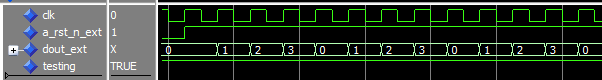
\includegraphics[width=1\textwidth]{img/Chapter4/counter.png}
    \caption{CounterTest}
    \label{fig:CounterTest}
\end{figure}

\subsection{Combinational Network Test}

In order to test the proper functioning of \textbf{Combinational Network}, an Excel file has been made, shown in the following figure: 

\begin{figure}[H]
    \centering
    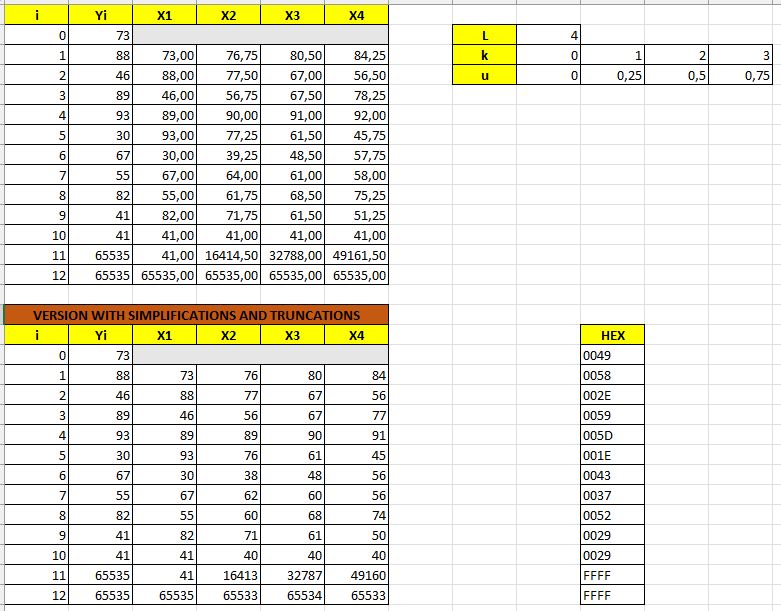
\includegraphics[width=0.8\textwidth]{img/Chapter4/Excel.png}
    \caption{Test Plan for Combinational Network}
    \label{fig:CNExcel1}
\end{figure}

In this file a series of values have been dynamically generated, and they are used to compute the linear interpolation with and without simplification (shift for division, etc...).

After that, some of this values are used to create the stimuli for the Combinational Network, in a test bench specifically created. The correctness of the results has been verified through a visual analysis. The ModelSim simulation obtained is the following:

\begin{figure}[H]
    \centering
    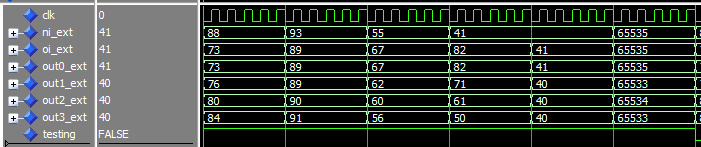
\includegraphics[width=1\textwidth]{img/Chapter4/CI.png}
    \caption{Combinational Network Test}
    \label{fig:CNTest}
\end{figure}

Moreover, in the Excel file there are both approximated and effective interpolated signals, so it is possible to compute the mean error, as shown below:

\begin{figure}[H]
    \centering
    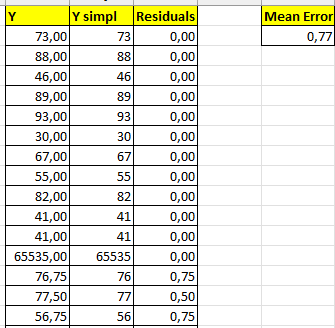
\includegraphics[width=0.4\textwidth]{img/Chapter4/Error.png}
    \caption{Mean Error caused by the simplifications}
    \label{fig:CNExcel2}
\end{figure}

It's clear that in this case the mean error is below one; This confirms the hypothesis that the error caused by the approximation is acceptable.

\subsection{Linear Interpolator Test}

As said before, the values obtained in the previous Excel file (Figure \ref{fig:CNExcel1}), has been used even in the \textbf{Linear Interpolator} test. The following figure represents the stimuli used in the test bench:

\begin{figure}[H]
    \centering
    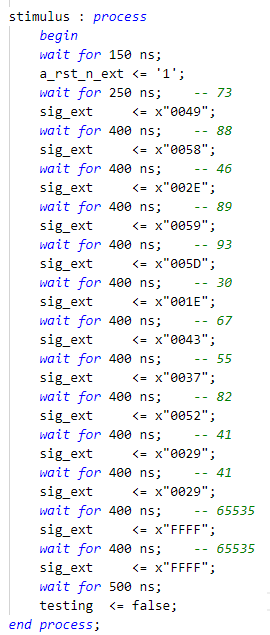
\includegraphics[width=0.3\textwidth]{img/Chapter4/Stimuli_Static.png}
    \caption{Stimuli for Linear Interpolator}
    \label{fig:LIStaticStimuli}
\end{figure}

Even in this case, the correctness of the results have been tested by a visual analysis, through the comparison with the Excel results.

\begin{figure}[H]
    \centering
    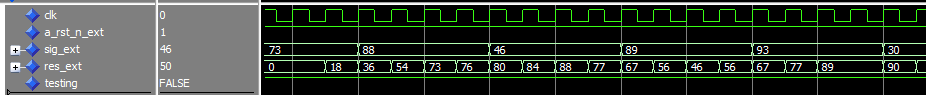
\includegraphics[width=1\textwidth]{img/Chapter4/LI_Static.png}
    \caption{Linear Interpolator First Test}
    \label{fig:LIStaticTest}
\end{figure}

In this test is possible to see that when a new signals arrives, the first of the four output signals is provided after two clock cycles. This delay is caused by the input registers and the output register that are between the input and the output of the network. 

\subsection{Linear Interpolator Dynamic Test}

As last step, a python script named \textit{TB\_Generation.py} has been created, that produces a test bench with a number of \textbf{dynamically generated stimuli}. This script takes in input as optional parameters the number of stimuli that have to generate, and the seed used for the generation (in order to have repeatable experiments).

\begin{figure}[H]
    \centering
    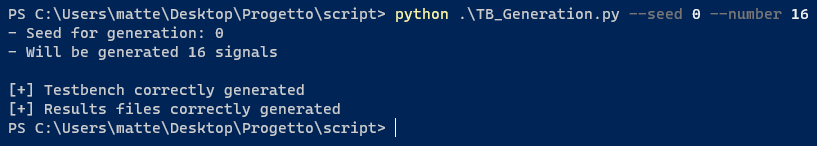
\includegraphics[width=1\textwidth]{img/Chapter4/script1.png}
    \caption{Script for Test bench Generation}
    \label{fig:Script1}
\end{figure}

The script generates three different files:

\begin{itemize}
    \item \textit{LinearInterpolator\_tb.vhd}, is generated the test bench.
    \item \textit{ExpectedResults.txt}, contains the list of the results that the circuit have to produce. It is used by a second script described below.
    \item \textit{TabulatedResults.txt}, contains the same results of previous file, but in a tabulated form, useful for an eventual visual analysis.
\end{itemize}

\begin{figure}[H]
    \centering
    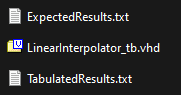
\includegraphics[width=0.4\textwidth]{img/Chapter4/GeneratedFiles.png}
    \caption{Generated Files}
    \label{fig:GenFiles}
\end{figure}

\newpage

Below there is an example of stimuli dinamically generated:

\begin{figure}[H]
    \centering
    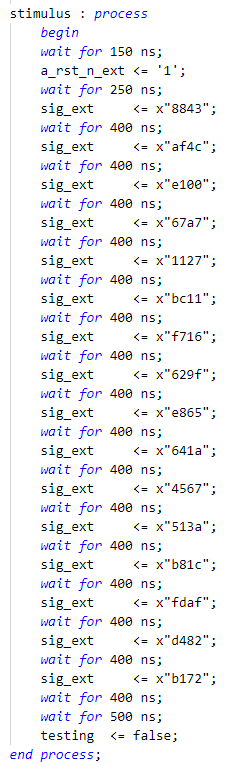
\includegraphics[width=0.4\textwidth]{img/Chapter4/GeneratedStimuli.png}
    \caption{Generated Stimuli}
    \label{fig:GenStimuli}
\end{figure}

\newpage

Instead, below there is an example of \textit{TabulatedResults.txt}:

\begin{figure}[H]
    \centering
    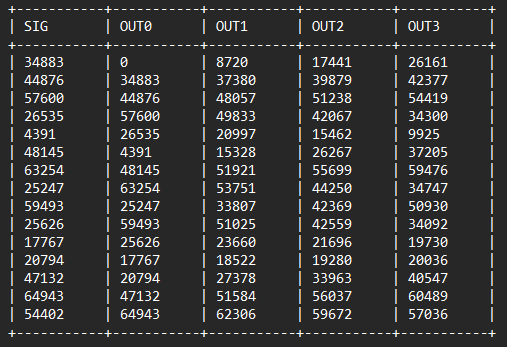
\includegraphics[width=0.6\textwidth]{img/Chapter4/ExpectedTabular.png}
    \caption{Expected Results in tabular form}
    \label{fig:ExpectedRes}
\end{figure}

The purpose of this system is to be able to test the circuit automatically and with a very large number of input signals.

For this purpose it is necessary to export from ModelSim the results obtained as output signals in a list.lst file, and run a second script (\textit{Results\_validator.py}) that compares the file exported from ModelSim with the results computed by the first script.

\begin{figure}[H]
    \centering
    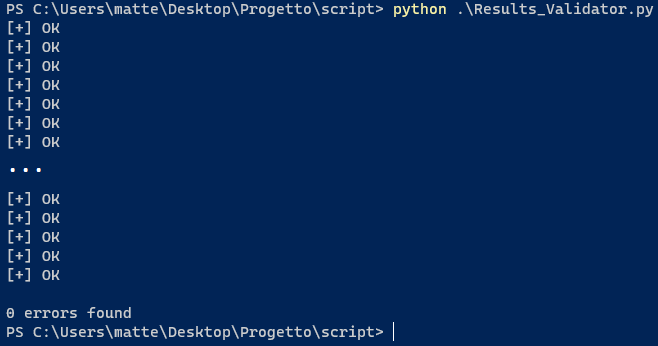
\includegraphics[width=0.6\textwidth]{img/Chapter4/Validator.png}
    \caption{Script for Results Validation}
    \label{fig:Script2}
\end{figure}

If the script finds errors, these will be notified as shown in the figure below:

\begin{figure}[H]
    \centering
    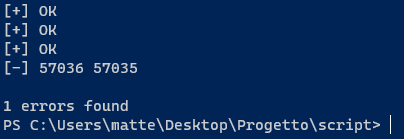
\includegraphics[width=0.6\textwidth]{img/Chapter4/Validator2.png}
    \caption{Example of wrong result}
    \label{fig:Script3}
\end{figure}
\section{Vivado Report}

In this last section an \textbf{automatic synthesis} will be done, through the tool \textbf{Xilinx Vivado}. The target working device is the FPGA \textit{xc7z010clg400-1} and the three steps that will be analyzed are the following:

\begin{enumerate}
    \item \textbf{Elaborated Design} Analysis.
    \item \textbf{Synthesis} and Report analysis.
    \item \textbf{Implementation} and Report analysis.
\end{enumerate}

\subsection{Elaborated Design Analysis}

In this first part will be analyzed the \textbf{Elaborated Design}, that is the Vivado representation of the Linear Interpolator at the \textbf{Register Transfer Level}. It should be equal to the structure defined in the  Architecture Description Section.

\begin{figure}[H]
    \centering
    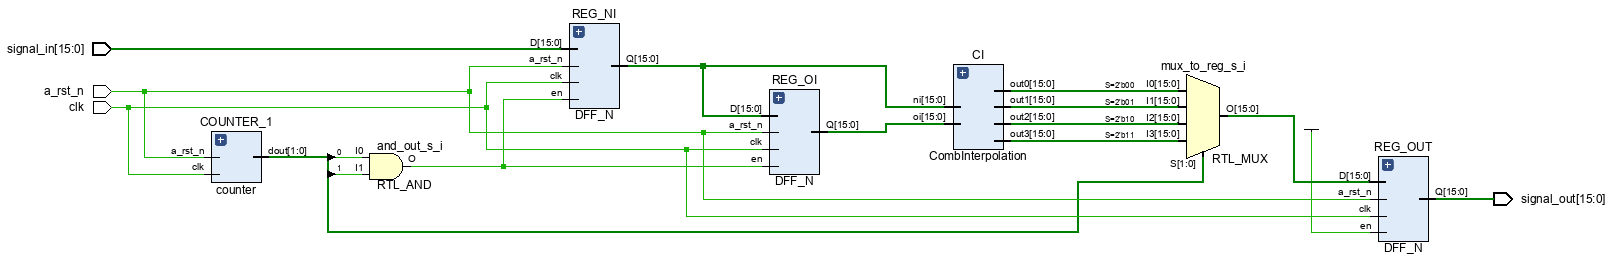
\includegraphics[width=1\textwidth]{img/Chapter5/Elaborated.png}
    \caption{Elaborated Design}
    \label{fig:ED}
\end{figure}

From the figure above is clear that the circuit respects the structure chosen in the planning stage, so it's possible to start the synthesis.

\subsection{Synthesis Analysis}

In this phase the Elaborated Design previously generated will be \textbf{translated} in circuits that the FPGA \textbf{can implement}. This will be done respecting all given \textbf{constraints}. In this case the only constraint is the clock, that must have a period of $8ns$.

The synthesis result is the following:

\begin{figure}[H]
    \centering
    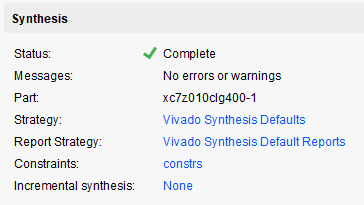
\includegraphics[width=0.5\textwidth]{img/Chapter5/SyntesisResult.png}
    \caption{Synthesis Result}
    \label{fig:SR}
\end{figure}

There are no errors or warnings, so it's possible to study the reports.

\subsubsection{Timing Report and Critical Path}

The \textbf{timings} obtained are as follows:

\begin{figure}[H]
    \centering
    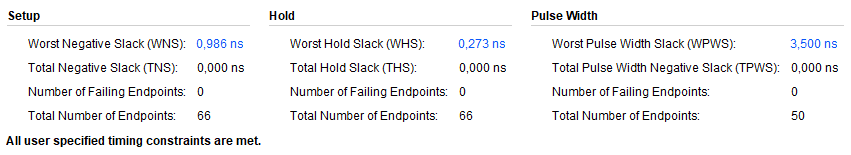
\includegraphics[width=1\textwidth]{img/Chapter5/SyntesisTiming.png}
    \caption{Timing Report}
    \label{fig:STR}
\end{figure}

First of all, there are \textbf{no negative slacks}, so the clock with a period of $8ns$ is clearly enough for the produced design. Moreover, the \textbf{worst negative slack} is $0.986ns$, so the clock can be at least faster of this value.

Analyzing the \textbf{synthesized design}, the \textbf{critical path} is the following:

\begin{figure}[H]
    \centering
    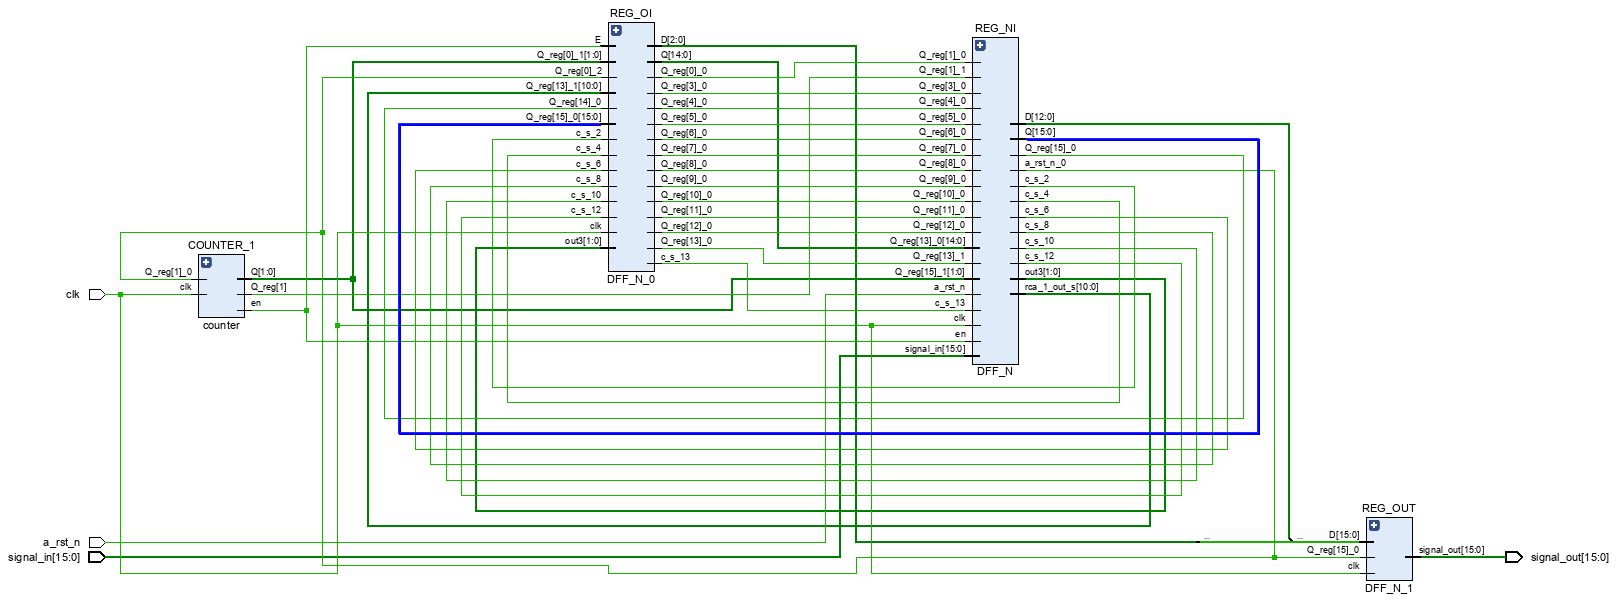
\includegraphics[width=1\textwidth]{img/Chapter5/SyntesisSetupCrit.png}
    \caption{Critical Path for Setup time}
    \label{fig:SCPS}
\end{figure}

\subsubsection{Utilization Analysis}

The \textbf{utilization report} obtained are as follows:

\begin{figure}[H]
    \centering
    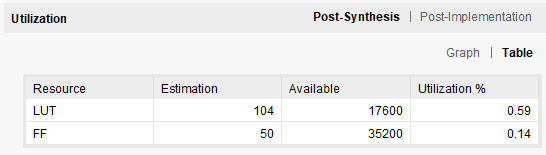
\includegraphics[width=0.6\textwidth]{img/Chapter5/SyntesisUtilization.png}
    \caption{Utilization Report}
    \label{fig:SU}
\end{figure}

The utilization for \textbf{Look Up Tables} and \textbf{Flip Flops} are lower then the $1\%$, so the FPGA has all resources needed to implement this circuit.

\subsubsection{Power Consumption Analysis}

The last report is about the \textbf{power consumption}. This is a very rough estimation, but allows to have a general idea of the circuit's power requirements.

\begin{figure}[H]
    \centering
    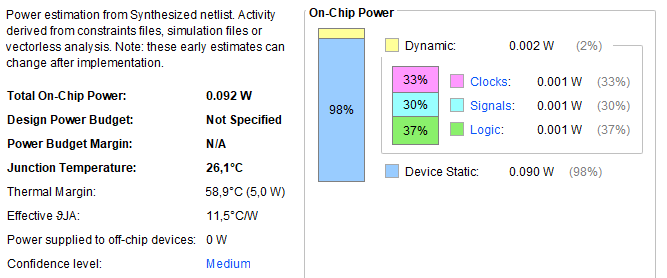
\includegraphics[width=1\textwidth]{img/Chapter5/SyntesisPower.png}
    \caption{Power Report}
    \label{fig:SPR}
\end{figure}

The \textbf{general consumption} is lower than  $100mW$. Moreover, it's clear that the percentage of static power is much greater than the dynamic power. So it's possible to say that the \textbf{switching activity} in this circuit is relatively low.

\subsection{Implementation analysis}

In this phase the \textbf{place and route} will be performed by Vivado, with some useful \textbf{optimizations}. In general this phase is preceded by the \textbf{I/O Planning}, in which the I/O Physical Ports of the FPGA are associated with the I/O Ports of the Elaborated Design. But the FPGA has not enough ports to implement an input and an output of 16 bit. So the implementation will be performed in \textit{Out of Context Mode}, that allows to do implementation without I/O Planning. 

The implementation result is the following:

\begin{figure}[H]
    \centering
    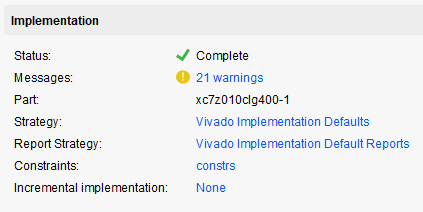
\includegraphics[width=0.5\textwidth]{img/Chapter5/ImplementationResult.png}
    \caption{Implementation Result}
    \label{fig:IR}
\end{figure}

There are no errors, but there are warnings. They will be analyzed later.

\subsubsection{Timing Report and Critical Path}

The \textbf{timings} obtained are as follows:

\begin{figure}[H]
    \centering
    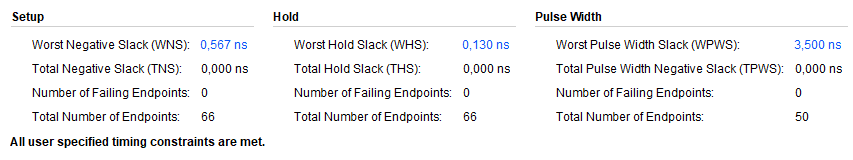
\includegraphics[width=1\textwidth]{img/Chapter5/ImplementationTiming.png}
    \caption{Timing Report}
    \label{fig:ITR}
\end{figure}

Even in this case there are \textbf{no negative slacks}, so a clock period of $8ns$ is fast enough. But in this case the \textbf{worst negative slack is worse} than before. This is due to the fact that the implementation allows to to obtain a more accurate estimate.

The \textbf{critical path} that cause this slack is the following:

\begin{figure}[H]
    \centering
    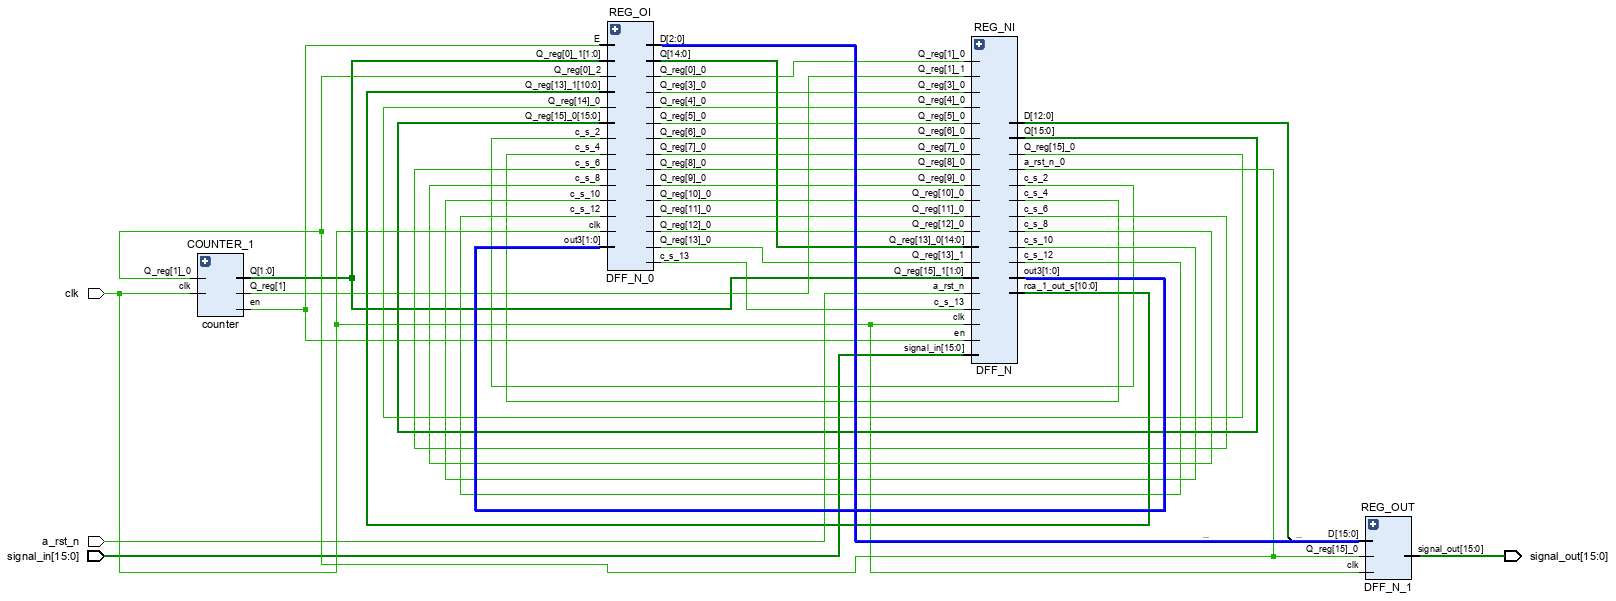
\includegraphics[width=1\textwidth]{img/Chapter5/ImplementationSetupCrit.png}
    \caption{Critical Path for Setup time}
    \label{fig:ICPS}
\end{figure}

\subsubsection{Utilization Analysis}

The \textbf{utilization report} obtained are as follows:

\begin{figure}[H]
    \centering
    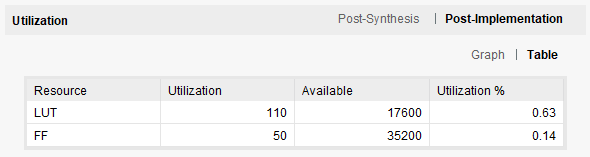
\includegraphics[width=0.6\textwidth]{img/Chapter5/ImplementationUtilization.png}
    \caption{Utilization Report}
    \label{fig:IU}
\end{figure}

Compared to the synthesis, the number of \textbf{Look Up Table} has increased to $110$, while the \textbf{Flip Flops} are the same.

\subsubsection{Power Consumption Analysis}

As regards power consumption, the results are the following:

\begin{figure}[H]
    \centering
    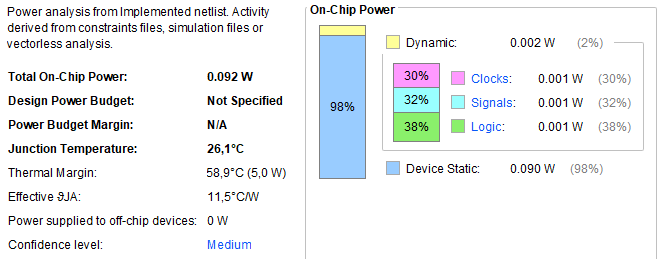
\includegraphics[width=1\textwidth]{img/Chapter5/ImplementationPower.png}
    \caption{Power Report}
    \label{fig:IPR}
\end{figure}

Compared to the synthesis, there are no changes.

\subsubsection{Warnings Analysis}

The Implementation's Warnings are the following:

\begin{figure}[H]
    \centering
    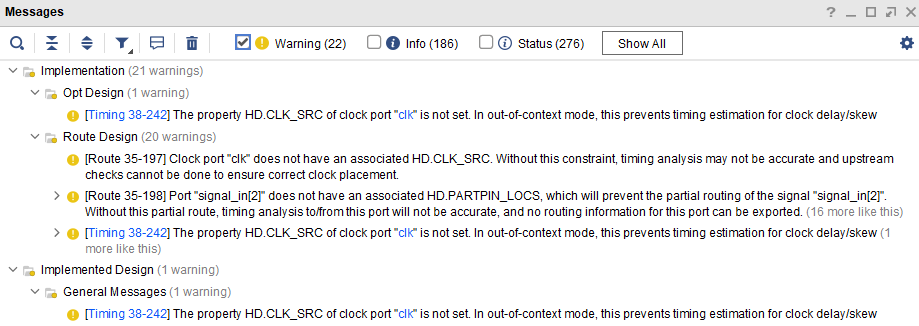
\includegraphics[width=1\textwidth]{img/Chapter5/ImplementationWarning.png}
    \caption{Implementation Warnings}
    \label{fig:IW}
\end{figure}

All of them are Vivado internal warnings, that can be ignored.
\section{Conclusions}

The \textbf{Linear Interpolator} is a circuit that, received two consecutive signals, provides in output the $L$ (factor of interpolation) signals that represent the linear interpolation between them.

Considering a circuit with a fixed L, there are many possible implementations, each of them allowing to get a different \textbf{trade-off} between \textbf{performance}, \textbf{complexity} and \textbf{precision}.

\begin{itemize}
    \item If an \textbf{high level of precision} is needed, the interpolation formula should not have any oversimplifications, so is necessary to implement multiplication and division modules (high complexity).
    \item If an \textbf{high speed} or \textbf{high power efficiency} is needed, a multiple clock domain should be implemented, obtaining an higher level of complexity.
    \item If a \textbf{low complexity} is needed, the proposed implementation should be chosen. In fact, it allows to implements the entire computation using unsigned signals and simple Ripple Carry Adders.
\end{itemize}

\end{document}
